\section{Results and Discussion}
% Talk about resulted data
% compare the different models results
% talk about the confusion matrix, talk about how the model is miss classifying some of the of the images as labels next to the original label, not too far away

Our research categorizes atmospheric visibility into five distinct categories, as summarized in Table~\ref{tab:vis_img_count}. This categorization is based on the visibility range in miles, which was set according to the requirements of the FAA. Resulting in a comprehensive dataset of 116,100 images spanning various altitudes, land covers, and sceneries.

The training of a single modality RGB model did not achieve high accuracy on the different classes of our problem, with an overall accuracy of 87.92\%. This demonstrates the limitations of such models, especially when tested on unseen views. Unlike previous works that were tested on a limited number of views and with a data split that might have caused data leakage between the training set and test set, our model may have given false results during evaluation as it had already seen a similar image during training. To prevent the same problem in our experiments, we used the holdout method as we mentioned in the Experimental Setup,  %TODO refer to the chapter
where we hide certain locations totally from the model during the training.



% \begin{figure}[htbp]
% \centerline{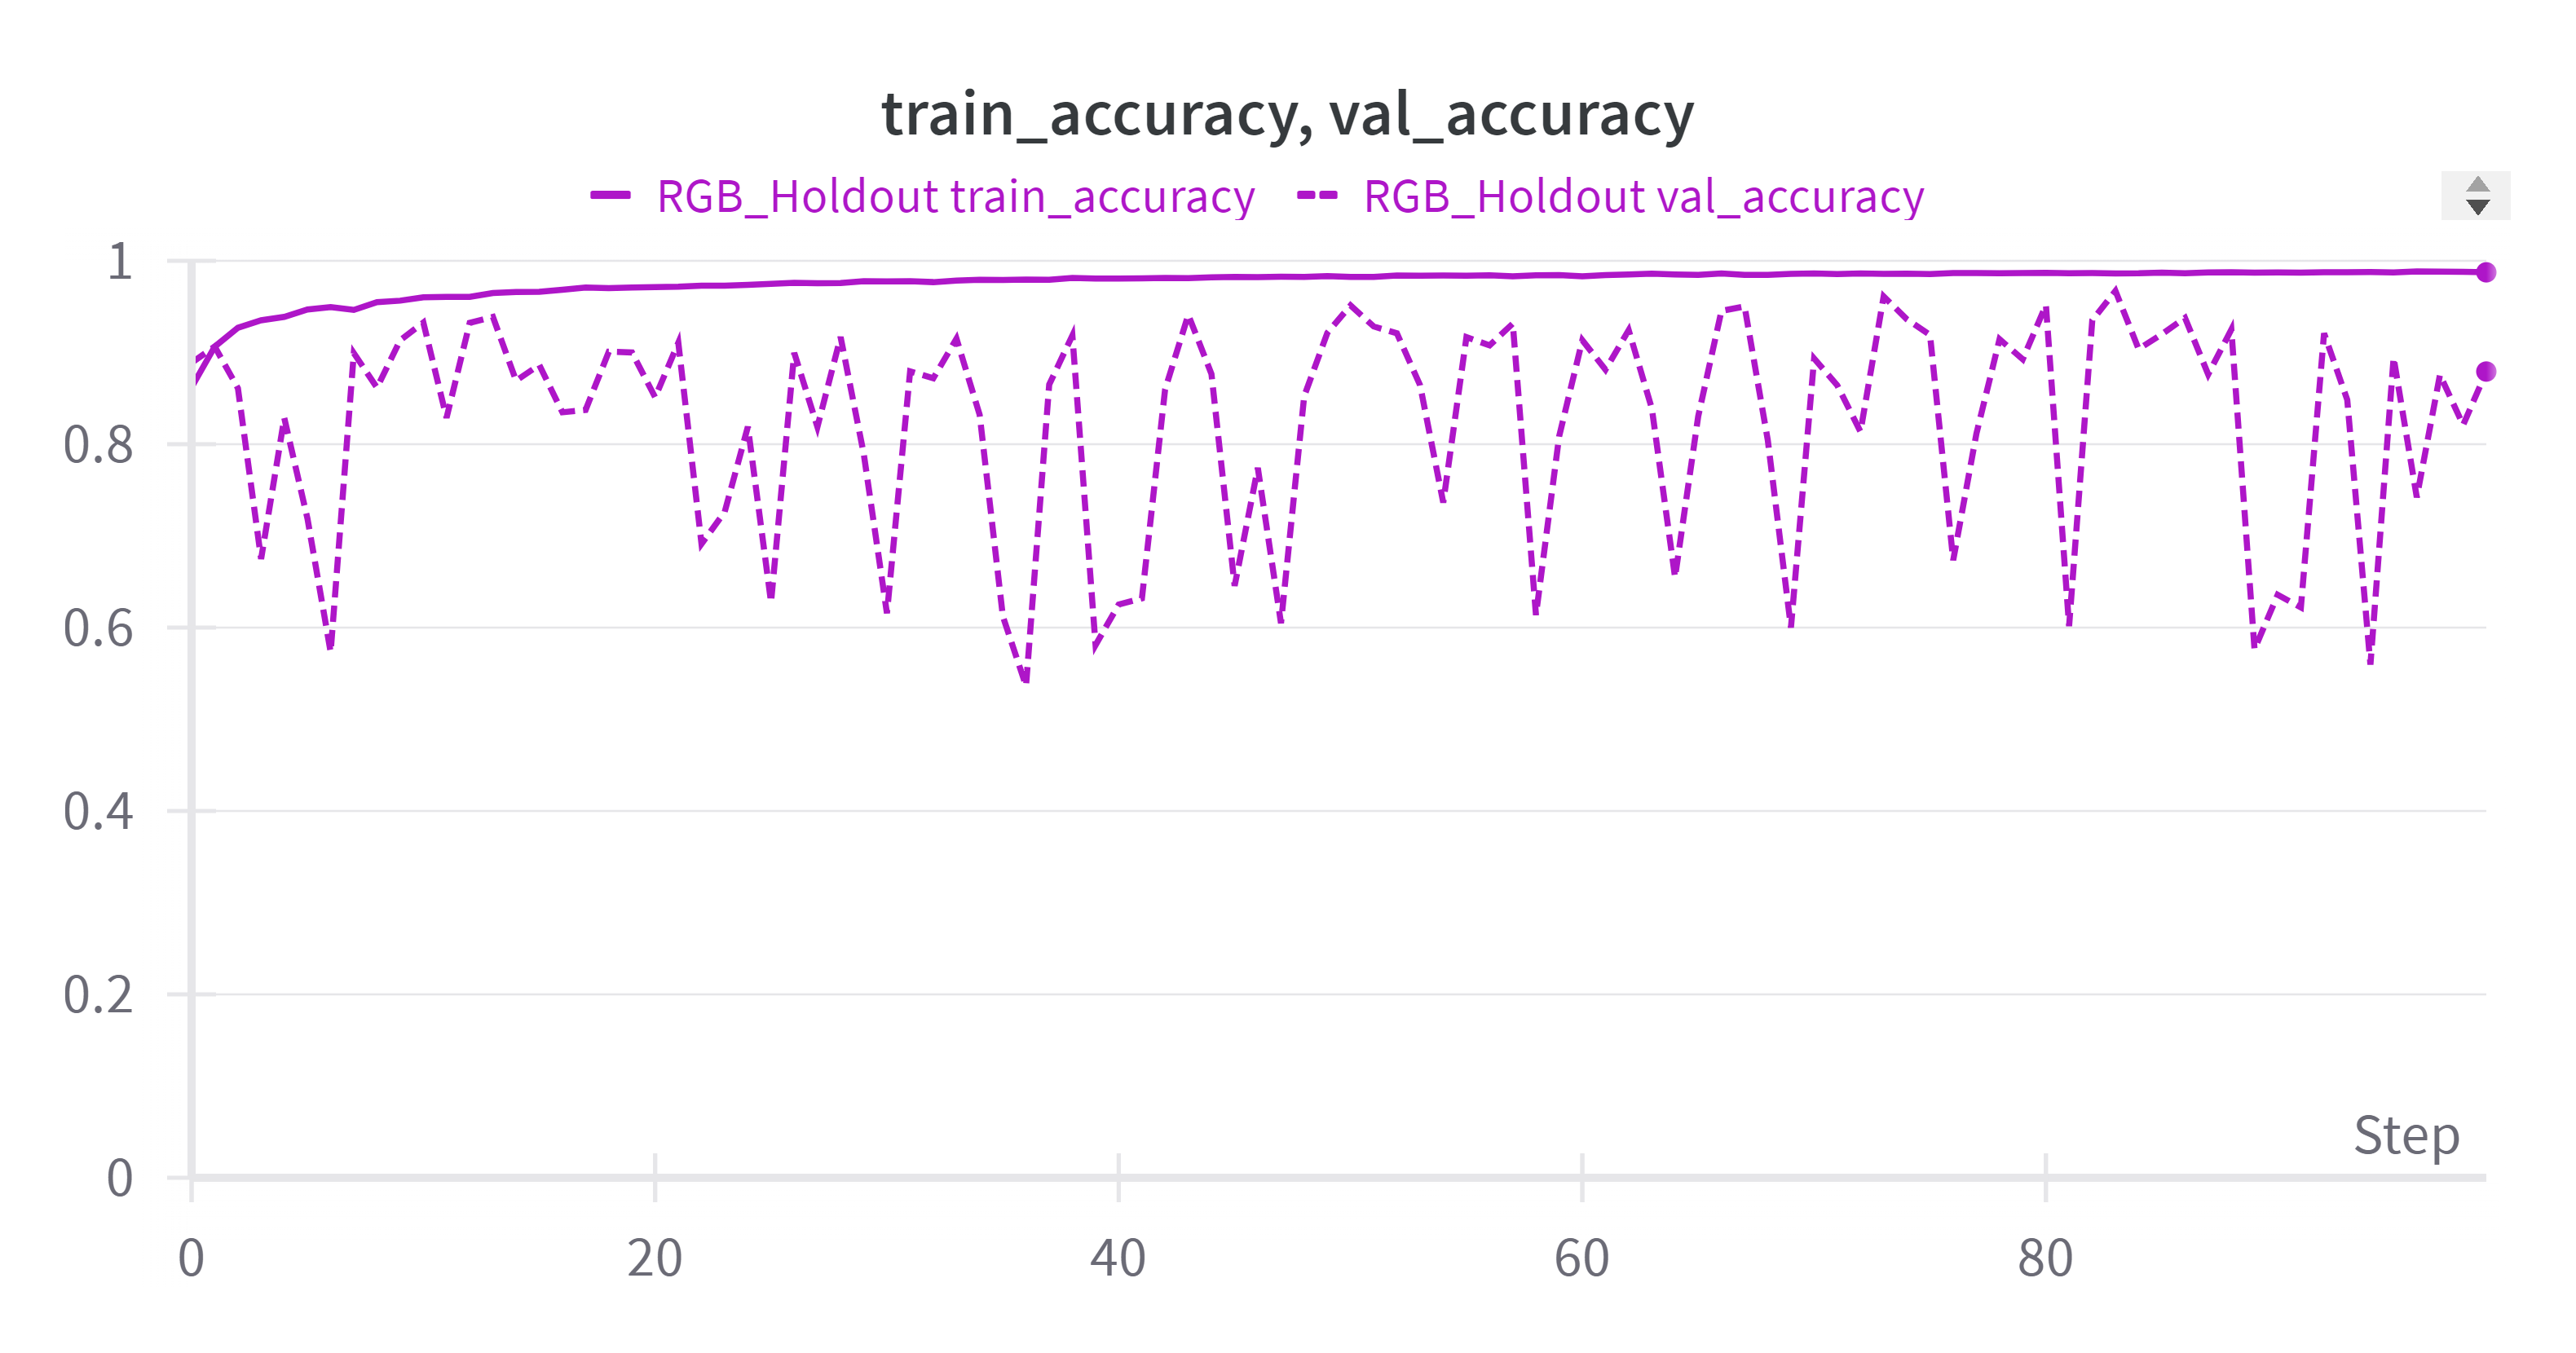
\includegraphics[width=250pt]{imgs/val_train_acc_rgb.png}}
% \caption{Training and Validation accuracy for RGB Model}
% \label{fig:rgb_model_training_history}
% \end{figure}

% \begin{figure}[htbp]
% \centerline{\includegraphics[width=250pt]{imgs/val_train_acc.png}}
% \caption{Training and Validation accuracy for RGB Model}
% \label{fig:rgb_model_training_history}
% \end{figure}


Unlike the single modality RGB model, results from the multimodality models (Table~\ref{tab:res_table}, Figure~\ref{fig:conf_mats})  show a big improvement in the accuracy of prediction in the validation set, compared with 87.92\% from the RGB model, when we fuse different modalities, we notice a leap of 10\% in accuracy. For instance, When we combine the embedding extracted from the RGB model with the embedding extracted from the depth map, the RGB-Depth model achieves a high accuracy of 96.53\% using a simple concatenate connector.


\begin{table*}

\centering
\caption{Results comparison of using different modalities, }
\begin{tabular}{c|c|c|c|c|c|c|c}
\hline
\label{tab:res_table}
Connector & RGB & Entropy & Edge & Depth &  Normal Surface  & \# trainable param & val acc.  \\
\hline
Unimodality & \checkmark &  &  &  &   &7M&  87.92  \\
% \multirow{5}{*}{Unimodality} & \checkmark &  &  &  &   &7M&  87.92  \\
% &  & \checkmark &&  &  &  7M &  95.6  \\
% &  &   & \checkmark &  &   &7M& 97.23  \\
% & &  &  & \checkmark &   &7M&   81.49  \\
% & &  &  &  & \checkmark  &7M&   85,68  \\
\hline

\multirow{5}{*}{Concatenate}& \checkmark & \checkmark &  &  &   &14M&  96.4  \\
& \checkmark &   & \checkmark &  &   &14M& 96.53   \\
& \checkmark &  &  & \checkmark &   &14M&   \textbf{97.57}  \\
% & \checkmark &  &  &  & \checkmark &$2*224^2$&14M&   In Training  \\
& \checkmark &  &  & \checkmark & \checkmark  &21M&   97.14  \\
& \checkmark & \checkmark & \checkmark  & \checkmark & \checkmark  & 38M & 96.3  \\
\hline
% \multirow{5}{*}{Self-Attention}& \checkmark & \checkmark &  &  &  &$2 * 224^2$&14M&  In-Training  \\
\multirow{4}{*}{Self-Attention} & \checkmark &   & \checkmark &  &   &14M& 96.86  \\
& \checkmark &  &  & \checkmark &   &14M&   96.31  \\
% & \checkmark &  &  &  & \checkmark &$2*224^2$&14M&   In-Training  \\
& \checkmark &  &  & \checkmark & \checkmark  &21M&   97.47  \\
& \checkmark & \checkmark & \checkmark  & \checkmark & \checkmark  & 38M & \textbf{97.63}  \\

\hline
\end{tabular}
\end{table*}
% End Table

% \begin{table*}

% \centering
% \caption{Results comparison of using different modalities, }
% \begin{tabular}{c|c|c|c|c|c|c|c|c}
% \hline
% \label{tab:res_table}
% Connector & RGB & Entropy & Edge & Depth &  Normal Surface & image size & \# trainable param & val acc.  \\
% \hline
% Single Modality & \checkmark &  &  &  &  &$224^2$&7M&  87.92  \\
% % &  & \checkmark &  &  &  &$224^2$&7M&  95.6  \\
% % &  &   & \checkmark &  &  &$224^2$&7M& 97.23  \\
% % & &  &  & \checkmark &  &$224^2$&7M&   81.49  \\
% % & &  &  &  & \checkmark &$224^2$&7M&   85,68  \\
% \hline

% \multirow{6}{*}{Concatenate}& \checkmark & \checkmark &  &  &  &$2 * 224^2$&14M&  96.4  \\
% & \checkmark &   & \checkmark &  &  &$2*224^2$&14M& 96.53   \\
% & \checkmark &  &  & \checkmark &  &$2*224^2$&14M&   \textbf{97.57}  \\
% % & \checkmark &  &  &  & \checkmark &$2*224^2$&14M&   In Training  \\
% & \checkmark &  &  & \checkmark & \checkmark &$3*224^2$&21M&   97.14  \\
% & \checkmark & \checkmark & \checkmark  & \checkmark & \checkmark &$5 * 224^2$& 38M & 96.3  \\
% \hline
% % \multirow{5}{*}{Self-Attention}& \checkmark & \checkmark &  &  &  &$2 * 224^2$&14M&  In-Training  \\
% \multirow{4}{*}{Self-Attention} & \checkmark &   & \checkmark &  &  &$2*224^2$&14M& 96.86  \\
% & \checkmark &  &  & \checkmark &  &$2*224^2$&14M&   96.31  \\
% % & \checkmark &  &  &  & \checkmark &$2*224^2$&14M&   In-Training  \\
% & \checkmark &  &  & \checkmark & \checkmark &$3*224^2$&21M&   97.47  \\
% & \checkmark & \checkmark & \checkmark  & \checkmark & \checkmark &$5 * 224^2$& 38M & \textbf{97.63}  \\

% \hline
% \end{tabular}
% \end{table*}
% % End Table


% Discussion
The confusion matrix and results table highlight the efficacy of multimodal deep learning in atmospheric visibility estimation for most of the categories (Figure~\ref{fig:conf_mats}). The overall performance is good, but the multimodality approach still struggles with label 3, which represents the visibility range from 3 to 5 miles. We've observed that all different combinations of modalities have difficulty with this class specifically, and most of them incorrectly predict it as class 4. Future work could focus on improving our solution for this specific class. The combination of RGB and Depth alone resulted in improved results in this specific class. This suggests that future research could focus on testing different modalities to achieve better results and reducing the number of modalities used to estimate visibility. This would help to reduce the computation cost of estimating visibility without negatively impacting the accuracy of the models.

\begin{figure}
    \centering
% Mean of Dark Channel Prior vs Visibility
    \begin{subfigure}[b]{0.4\textwidth}
    %The matrix in numbers
%Horizontal target class
%Vertical output class
\def\myConfMat{{
{669,   3,   0,   0,    0},  %row 1
{  3,  657,  0,   0,    0},  %row 2
{   0,  12, 2638,  85,    33},  %row 3
{   0,   0,  50, 2368,   56},  %row 4
{   0,   0,   0,  132, 8941},  %row 5
}}

\def\classNames{{"$0$","$1$","$2$","$3$","$4$"}} %class names. Adapt at will

\def\numClasses{5} %number of classes. Could be automatic, but you can change it for tests.

\def\myScale{1.05} % 1.5 is a good scale. Values under 1 may need smaller fonts!
\begin{tikzpicture}[
    scale = \myScale,
    %font={\scriptsize}, %for smaller scales, even \tiny may be useful
    ]

\tikzset{vertical label/.style={rotate=90,anchor=east}}   % usable styles for below
\tikzset{diagonal label/.style={rotate=45,anchor=north east}}

\foreach \y in {1,...,\numClasses} %loop vertical starting on top
{
    % Add class name on the left
    \node [anchor=east] at (0.4,-\y) {\pgfmathparse{\classNames[\y-1]}\pgfmathresult}; 
    
    \foreach \x in {1,...,\numClasses}  %loop horizontal starting on left
    {
%---- Start of automatic calculation of totSamples for the column ------------   
    \def\totSamples{0}
    \foreach \ll in {1,...,\numClasses}
    {
        \pgfmathparse{\myConfMat[\ll-1][\x-1]}   %fetch next element
        \xdef\totSamples{\totSamples+\pgfmathresult} %accumulate it with previous sum
        %must use \xdef fro global effect otherwise lost in foreach loop!
    }
    \pgfmathparse{\totSamples} \xdef\totSamples{\pgfmathresult}  % put the final sum in variable
%---- End of automatic calculation of totSamples ----------------
    
    \begin{scope}[shift={(\x,-\y)}]
        \def\mVal{\myConfMat[\y-1][\x-1]} % The value at index y,x (-1 because of zero indexing)
        \pgfmathtruncatemacro{\r}{\mVal}   %
        \pgfmathtruncatemacro{\p}{round(\r/\totSamples*100)}
        \coordinate (C) at (0,0);
        \ifthenelse{\p<50}{\def\txtcol{black}}{\def\txtcol{white}} %decide text color for contrast
        \node[
            draw,                 %draw lines
            text=\txtcol,         %text color (automatic for better contrast)
            align=center,         %align text inside cells (also for wrapping)
            fill=black!\p,        %intensity of fill (can change base color)
            minimum size=\myScale*10mm,    %cell size to fit the scale and integer dimensions (in cm)
            inner sep=0,          %remove all inner gaps to save space in small scales
            ] (C) {\r\\\p\%};     %text to put in cell (adapt at will)
        %Now if last vertical class add its label at the bottom
        \ifthenelse{\y=\numClasses}{
        \node [] at ($(C)-(0,0.75)$) % can use vertical or diagonal label as option
        {\pgfmathparse{\classNames[\x-1]}\pgfmathresult};}{}
    \end{scope}
    }
}
%Now add x and y labels on suitable coordinates
\coordinate (yaxis) at (-0.2,0.3-\numClasses/2);  %must adapt if class labels are wider!
\coordinate (xaxis) at (0.5+\numClasses/2, -\numClasses-1.2); %id. for non horizontal labels!
\node [vertical label] at (yaxis) {Predicted Label};
\node []               at (xaxis) {True Label};
\end{tikzpicture}

\caption{All modalities with the Self-Attention Block}

    
    % 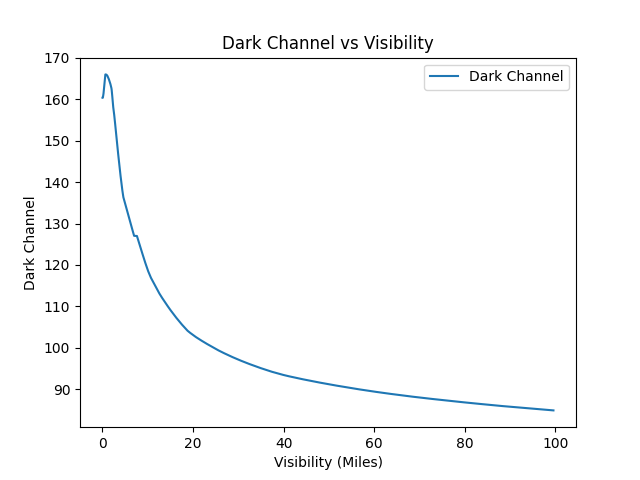
\includegraphics[width=\textwidth]{imgs/dark_channel_vs_visibility.png}
    \end{subfigure}
    % Mean of Dark Channel Prior vs Visibility
    \begin{subfigure}[b]{0.4\textwidth}
        %The matrix in numbers
%Horizontal target class
%Vertical output class
\def\myConfMat{{
{664,   0,   0,   0,    0},  %row 1
{  8,  663,  0,   0,    0},  %row 2
{   0,  9, 2618,  143,    114},  %row 3
{   0,   0,  70, 2368,   61},  %row 4
{   0,   0,   0,  177, 8855},  %row 5
}}

\def\classNames{{"$0$","$1$","$2$","$3$","$4$"}} %class names. Adapt at will

\def\numClasses{5} %number of classes. Could be automatic, but you can change it for tests.

\def\myScale{1.05} % 1.5 is a good scale. Values under 1 may need smaller fonts!
\begin{tikzpicture}[
    scale = \myScale,
    %font={\scriptsize}, %for smaller scales, even \tiny may be useful
    ]

\tikzset{vertical label/.style={rotate=90,anchor=east}}   % usable styles for below
\tikzset{diagonal label/.style={rotate=45,anchor=north east}}

\foreach \y in {1,...,\numClasses} %loop vertical starting on top
{
    % Add class name on the left
    \node [anchor=east] at (0.4,-\y) {\pgfmathparse{\classNames[\y-1]}\pgfmathresult}; 
    
    \foreach \x in {1,...,\numClasses}  %loop horizontal starting on left
    {
%---- Start of automatic calculation of totSamples for the column ------------   
    \def\totSamples{0}
    \foreach \ll in {1,...,\numClasses}
    {
        \pgfmathparse{\myConfMat[\ll-1][\x-1]}   %fetch next element
        \xdef\totSamples{\totSamples+\pgfmathresult} %accumulate it with previous sum
        %must use \xdef fro global effect otherwise lost in foreach loop!
    }
    \pgfmathparse{\totSamples} \xdef\totSamples{\pgfmathresult}  % put the final sum in variable
%---- End of automatic calculation of totSamples ----------------
    
    \begin{scope}[shift={(\x,-\y)}]
        \def\mVal{\myConfMat[\y-1][\x-1]} % The value at index y,x (-1 because of zero indexing)
        \pgfmathtruncatemacro{\r}{\mVal}   %
        \pgfmathtruncatemacro{\p}{round(\r/\totSamples*100)}
        \coordinate (C) at (0,0);
        \ifthenelse{\p<50}{\def\txtcol{black}}{\def\txtcol{white}} %decide text color for contrast
        \node[
            draw,                 %draw lines
            text=\txtcol,         %text color (automatic for better contrast)
            align=center,         %align text inside cells (also for wrapping)
            fill=black!\p,        %intensity of fill (can change base color)
            minimum size=\myScale*10mm,    %cell size to fit the scale and integer dimensions (in cm)
            inner sep=0,          %remove all inner gaps to save space in small scales
            ] (C) {\r\\\p\%};     %text to put in cell (adapt at will)
        %Now if last vertical class add its label at the bottom
        \ifthenelse{\y=\numClasses}{
        \node [] at ($(C)-(0,0.75)$) % can use vertical or diagonal label as option
        {\pgfmathparse{\classNames[\x-1]}\pgfmathresult};}{}
    \end{scope}
    }
}
%Now add x and y labels on suitable coordinates
\coordinate (yaxis) at (-0.2,0.3-\numClasses/2);  %must adapt if class labels are wider!
\coordinate (xaxis) at (0.5+\numClasses/2, -\numClasses-1.2); %id. for non horizontal labels!
\node [vertical label] at (yaxis) {Predicted Label};
\node []               at (xaxis) {True Label};
\end{tikzpicture}

\caption{All modalities with the concatenate connector}

    \end{subfigure}
    % Mean of Edge Density vs Visibility
    \begin{subfigure}[b]{0.4\textwidth}
        %The matrix in numbers
%Horizontal target class
%Vertical output class
\def\myConfMat{{
{660,   0,   0,   0,    0},  %row 1
{  12,  671,  41,   0,    0},  %row 2
{   0,  1, 2540,  23,    0},  %row 3
{   0,   0,  107, 2524,   57},  %row 4
{   0,   0,   0,  141, 8973},  %row 5
}}

\def\classNames{{"$0$","$1$","$2$","$3$","$4$"}} %class names. Adapt at will

\def\numClasses{5} %number of classes. Could be automatic, but you can change it for tests.

\def\myScale{1.05} % 1.5 is a good scale. Values under 1 may need smaller fonts!
\begin{tikzpicture}[
    scale = \myScale,
    %font={\scriptsize}, %for smaller scales, even \tiny may be useful
    ]

\tikzset{vertical label/.style={rotate=90,anchor=east}}   % usable styles for below
\tikzset{diagonal label/.style={rotate=45,anchor=north east}}

\foreach \y in {1,...,\numClasses} %loop vertical starting on top
{
    % Add class name on the left
    \node [anchor=east] at (0.4,-\y) {\pgfmathparse{\classNames[\y-1]}\pgfmathresult}; 
    
    \foreach \x in {1,...,\numClasses}  %loop horizontal starting on left
    {
%---- Start of automatic calculation of totSamples for the column ------------   
    \def\totSamples{0}
    \foreach \ll in {1,...,\numClasses}
    {
        \pgfmathparse{\myConfMat[\ll-1][\x-1]}   %fetch next element
        \xdef\totSamples{\totSamples+\pgfmathresult} %accumulate it with previous sum
        %must use \xdef fro global effect otherwise lost in foreach loop!
    }
    \pgfmathparse{\totSamples} \xdef\totSamples{\pgfmathresult}  % put the final sum in variable
%---- End of automatic calculation of totSamples ----------------
    
    \begin{scope}[shift={(\x,-\y)}]
        \def\mVal{\myConfMat[\y-1][\x-1]} % The value at index y,x (-1 because of zero indexing)
        \pgfmathtruncatemacro{\r}{\mVal}   %
        \pgfmathtruncatemacro{\p}{round(\r/\totSamples*100)}
        \coordinate (C) at (0,0);
        \ifthenelse{\p<50}{\def\txtcol{black}}{\def\txtcol{white}} %decide text color for contrast
        \node[
            draw,                 %draw lines
            text=\txtcol,         %text color (automatic for better contrast)
            align=center,         %align text inside cells (also for wrapping)
            fill=black!\p,        %intensity of fill (can change base color)
            minimum size=\myScale*10mm,    %cell size to fit the scale and integer dimensions (in cm)
            inner sep=0,          %remove all inner gaps to save space in small scales
            ] (C) {\r\\\p\%};     %text to put in cell (adapt at will)
        %Now if last vertical class add its label at the bottom
        \ifthenelse{\y=\numClasses}{
        \node [] at ($(C)-(0,0.75)$) % can use vertical or diagonal label as option
        {\pgfmathparse{\classNames[\x-1]}\pgfmathresult};}{}
    \end{scope}
    }
}
%Now add x and y labels on suitable coordinates
\coordinate (yaxis) at (-0.2,0.3-\numClasses/2);  %must adapt if class labels are wider!
\coordinate (xaxis) at (0.5+\numClasses/2, -\numClasses-1.2); %id. for non horizontal labels!
\node [vertical label] at (yaxis) {Predicted Label};
\node []               at (xaxis) {True Label};
\end{tikzpicture}

\caption{RGB and Depth Map Model with the Concatenate Connector}
    
    \end{subfigure}
    % Mean of FFT Magnitude vs Visibility
    \begin{subfigure}[b]{0.4\textwidth}
        %The matrix in numbers
%Horizontal target class
%Vertical output class
\def\myConfMat{{
{635,   0,   0,   0,    0},  %row 1
{  37,  661,  0,   0,    0},  %row 2
{   0,  11, 2636,  52,    0},  %row 3
{   0,   0,  52, 2301,   307},  %row 4
{   0,   0,   0,  94, 8936},  %row 5
}}

\def\classNames{{"$0$","$1$","$2$","$3$","$4$"}} %class names. Adapt at will

\def\numClasses{5} %number of classes. Could be automatic, but you can change it for tests.

\def\myScale{1.05} % 1.5 is a good scale. Values under 1 may need smaller fonts!
\begin{tikzpicture}[
    scale = \myScale,
    %font={\scriptsize}, %for smaller scales, even \tiny may be useful
    ]

\tikzset{vertical label/.style={rotate=90,anchor=east}}   % usable styles for below
\tikzset{diagonal label/.style={rotate=45,anchor=north east}}

\foreach \y in {1,...,\numClasses} %loop vertical starting on top
{
    % Add class name on the left
    \node [anchor=east] at (0.4,-\y) {\pgfmathparse{\classNames[\y-1]}\pgfmathresult}; 
    
    \foreach \x in {1,...,\numClasses}  %loop horizontal starting on left
    {
%---- Start of automatic calculation of totSamples for the column ------------   
    \def\totSamples{0}
    \foreach \ll in {1,...,\numClasses}
    {
        \pgfmathparse{\myConfMat[\ll-1][\x-1]}   %fetch next element
        \xdef\totSamples{\totSamples+\pgfmathresult} %accumulate it with previous sum
        %must use \xdef fro global effect otherwise lost in foreach loop!
    }
    \pgfmathparse{\totSamples} \xdef\totSamples{\pgfmathresult}  % put the final sum in variable
%---- End of automatic calculation of totSamples ----------------
    
    \begin{scope}[shift={(\x,-\y)}]
        \def\mVal{\myConfMat[\y-1][\x-1]} % The value at index y,x (-1 because of zero indexing)
        \pgfmathtruncatemacro{\r}{\mVal}   %
        \pgfmathtruncatemacro{\p}{round(\r/\totSamples*100)}
        \coordinate (C) at (0,0);
        \ifthenelse{\p<50}{\def\txtcol{black}}{\def\txtcol{white}} %decide text color for contrast
        \node[
            draw,                 %draw lines
            text=\txtcol,         %text color (automatic for better contrast)
            align=center,         %align text inside cells (also for wrapping)
            fill=black!\p,        %intensity of fill (can change base color)
            minimum size=\myScale*10mm,    %cell size to fit the scale and integer dimensions (in cm)
            inner sep=0,          %remove all inner gaps to save space in small scales
            ] (C) {\r\\\p\%};     %text to put in cell (adapt at will)
        %Now if last vertical class add its label at the bottom
        \ifthenelse{\y=\numClasses}{
        \node [] at ($(C)-(0,0.75)$) % can use vertical or diagonal label as option
        {\pgfmathparse{\classNames[\x-1]}\pgfmathresult};}{}
    \end{scope}
    }
}
%Now add x and y labels on suitable coordinates
\coordinate (yaxis) at (-0.2,0.3-\numClasses/2);  %must adapt if class labels are wider!
\coordinate (xaxis) at (0.5+\numClasses/2, -\numClasses-1.2); %id. for non horizontal labels!
\node [vertical label] at (yaxis) {Predicted Label};
\node []               at (xaxis) {True Label};
\end{tikzpicture}

\caption{RGB and Depth Map Model with the Self-Attention Block}
    
    \end{subfigure}
    \caption{Confusion Matrix of the top 4 multimodality models}
    \label{fig:conf_mats}
\end{figure}


Another perspective that should be considered when deciding which modality you want to use for the visibility estimation is the computation cost required to run the inference, while the model that merged all the available modalities gave us the best results, it still requires passing the input to all the modality estimators and then to the backbones, which makes it require more resources. and when planning to deploy such models, you will start facing the limits to what your hardware can give, so you need to consider that, especially for embedded devices.

While our dataset addressed the gap in the availability of publicly accessible multi-view datasets for atmospheric visibility, one of its limitations is the lack of diversity in landscapes and land covers. While experiments were conducted to ensure that there was no data leakage and that the model was tested on unseen locations, there is still a need to improve the quality of such a dataset by using the latest simulator technologies such as Microsoft Flight Simulator, X-Plane 12 that provides near real-world simulations for visibility degradation, which will help tackle the lack of available datasets.

Future research should focus on diversifying the dataset, incorporating a wider range of atmospheric conditions and scenarios. This expansion is not just about quantity, but also about variety, ensuring the SeeNN framework is tested against different visibility situations. Adding different land covers will enrich the dataset, making the model more adaptable to varying geographical locations and environmental conditions.

Another future work will be the use of the different pretraining techniques used in the literature to improve representation extracted from the different images, as similar to our work, most of the multimodal works make the use of the advancement of task-specific models to generate pseudo labels that are used to pre-train the model in an unsupervised manner, removing the need of requiring labeled data.

Furthermore, we found the need to understand how the different visibility degradations impact the quality of features extracted features by the different architectures, successfully understanding this point will help us in improving the trustworthiness of such models in real-world situations and not only reliable for sandbox situations.



